\documentclass{article}

\usepackage[utf8]{inputenc}
\usepackage[T1]{fontenc}
\usepackage[ngerman]{babel}
\usepackage{amsmath, amsfonts, amsthm, mathtools, amssymb}
\usepackage{stmaryrd}
\usepackage{enumerate}
\usepackage{cases}
\usepackage{fancyhdr}
\usepackage{comment}
%\usepackage{xcolor}
\usepackage{tikz}
\usepackage{pgf}
\usepackage{pgfplots}
\pgfplotsset{compat=1.16}
\usepackage{cases}
\usepackage{listings}
\usepackage{siunitx}
\usepackage[left = 3cm, bottom =3cm]{geometry}
\usepackage[hidelinks]{hyperref}
\usepackage{subcaption}
\usepackage{gauss}
\usepackage{nicematrix}

\usepackage{environ}
\newtheorem{satz}{Satz}[section]
\newtheorem{lemma}[satz]{Lemma}
\newtheorem{korollar}[satz]{Korollar}
\newtheorem{proposition}[satz]{Proposition}
\theoremstyle{definition}
\newtheorem{definition}[satz]{Def.}
\newtheorem{axiom}[satz]{Axiom}
\newtheorem{bsp}[satz]{Bsp.}
\newtheorem*{anmerkung}{Anm}
\newtheorem{bemerkung}[satz]{Bem}
\newtheorem*{notatio}{Notation}
\newcommand{\obda}{O.B.d.A. }
\newcommand{\equals}{\Longleftrightarrow}
\newcommand{\N}{\mathbb{N}}
\newcommand{\Q}{\mathbb{Q}}
\newcommand{\R}{\mathbb{R}}
\newcommand{\Z}{\mathbb{Z}}
\newcommand{\C}{\mathbb{C}}
\newcommand{\K}{\mathbb{K}}
\newcommand{\intd}{\mathrm{d}}
\newcommand{\Pot}{\operatorname{Pot}}
\newcommand{\mychar}{\operatorname{char}}
\newcommand{\myker}{\operatorname{ker}}
\newcommand{\induktion}[3]
{\begin{proof}\ \\
	\noindent\textbf{Induktionsanfang:}\ #1\\
	\noindent\textbf{Induktionsvoraussetzung:}\ #2\\
	\noindent\textbf{Induktionsschluss:}\ #3
\end{proof}}

\newcommand{\rg}{\operatorname{rg}}
\newcommand{\im}{\operatorname{im}}
\newcommand{\End}{\operatorname{End}}
\newcommand{\abb}{\operatorname{Abb}}
\newcommand{\re}{\operatorname{Re}}
\newcommand{\Ima}{\operatorname{Im}}

\let\oldstackrel\stackrel
\renewcommand{\stackrel}[2]{%
    \oldstackrel{\mathclap{#1}}{#2}
}%


\newcommand{\numlayout}[1]
{	
	\pagestyle{fancy}
	\fancyhead[L]{Einführung in die Numerik, Blatt #1}
	\fancyhead[R]{David Wesner, Josua Kugler}
	\fancypagestyle{firstpage}{%
		\fancyhf{}
		\lhead{Professor: Peter Bastian\\
			Tutor: Ernestine Großmann}
		\rhead{Einführung in die Numerik, Übungsblatt #1\\ David, Josua}
		\cfoot{\thepage}
	}
\thispagestyle{firstpage}
}

\newcommand{\analayout}[1]
{	
	\pagestyle{fancy}
	\fancyhead[L]{Analysis 2, Blatt #1}
	\fancyhead[R]{David Wesner, Josua Kugler}
	\fancypagestyle{firstpage}{%
		\fancyhf{}
		\lhead{Professor: Ekaterina Kostina\\
			Tutor: Julian Matthes}
		\rhead{Analysis 1, Übungsblatt #1\\ David Wesner, Josua Kugler}
		\cfoot{\thepage}
	}
	\thispagestyle{firstpage}
}
\newcommand{\lalayout}[1]
{	
	\pagestyle{fancy}
	\fancyhead[L]{Lineare Algebra 2, Blatt #1}
	\fancyhead[R]{David Wesner, Josua Kugler}
	\fancypagestyle{firstpage}{%
		\fancyhf{}
		\lhead{Professor: Denis Vogel\\
			Tutor: Marina Savarino}
		\rhead{Lineare Algebra 2, Übungsblatt #1\\ David Wesner, Josua Kugler}
		\cfoot{\thepage}
	}
	\thispagestyle{firstpage}
}

\lstset{
    frame=tb, % draw a frame at the top and bottom of the code block
    tabsize=4, % tab space width
    showstringspaces=false, % don't mark spaces in strings
    numbers=left, % display line numbers on the left
    commentstyle=\color{green}, % comment color
    keywordstyle=\color{blue}, % keyword color
    stringstyle=\color{red} % string color
}
\setlength{\headheight}{25pt}

\makeatletter \renewcommand\d{\ensuremath{%
		\;\mathrm{d}}}
\makeatother

\ExplSyntaxOn

% S-tackrelcompatible ALIGN environment
% some might also call it the S-uper ALIGN environment
% uses regular expressions to calculate the widest stackrel
% to put additional padding on both sides of relation symbols
\NewEnviron{salign}
{
    \begin{align}
        \lec_insert_padding:V \BODY
    \end{align}
}
% starred version that does no equation numbering
\NewEnviron{salign*}
{
    \begin{align*}
        \lec_insert_padding:V \BODY
    \end{align*}
}

% some helper variables
\tl_new:N \l__lec_text_tl
\seq_new:N \l_lec_stackrels_seq
\int_new:N \l_stackrel_count_int
\int_new:N \l_idx_int
\box_new:N \l_tmp_box
\dim_new:N \l_tmp_dim_a
\dim_new:N \l_tmp_dim_b
\dim_new:N \l_tmp_dim_needed

% function to insert padding according to widest stackrel
\cs_new_protected:Nn \lec_insert_padding:n
 {
  \tl_set:Nn \l__lec_text_tl { #1 }
  % get all stackrels in this align environment
  \regex_extract_all:nnN { \c{stackrel}{(.*?)}{(.*?)} } { #1 } \l_lec_stackrels_seq
  % get number of stackrels
  \int_set:Nn \l_stackrel_count_int { \seq_count:N \l_lec_stackrels_seq }
  \int_set:Nn \l_idx_int { 1 }
  \dim_set:Nn \l_tmp_dim_needed { 0pt }
  % iterate over stackrels
  \int_while_do:nn { \l_idx_int <= \l_stackrel_count_int }
  {
      % calculate width of text
      \hbox_set:Nn \l_tmp_box {$\seq_item:Nn \l_lec_stackrels_seq { \l_idx_int + 1 }$}
      \dim_set:Nn \l_tmp_dim_a {\box_wd:N \l_tmp_box}
      % calculate width of relation symbol
      \hbox_set:Nn \l_tmp_box {$\seq_item:Nn \l_lec_stackrels_seq { \l_idx_int + 2 }$}
      \dim_set:Nn \l_tmp_dim_b {\box_wd:N \l_tmp_box}
      % check if 0.5*(a-b) > minimum padding, if yes updated minimum padding
      \dim_compare:nNnTF
        { 1pt * \dim_ratio:nn { \l_tmp_dim_a - \l_tmp_dim_b } { 2pt } } > { \l_tmp_dim_needed }
        { \dim_set:Nn \l_tmp_dim_needed { 1pt * \dim_ratio:nn { \l_tmp_dim_a - \l_tmp_dim_b } { 2pt } } }
        { }
      \quad
      % increment list index by three, as every stackrel produces three list entries
      \int_incr:N \l_idx_int
      \int_incr:N \l_idx_int
      \int_incr:N \l_idx_int
  }
  % replace all relations with align characters (&) and add the needed padding
  \regex_replace_all:nnN
      { (\c{approx}&|&\c{approx}|\c{equiv}&|&\c{equiv}|=&|&=|\c{le}&|&\c{le}|\c{ge}&|&\c{ge}|&\c{stackrel}{.*?}{.*?}|\c{stackrel}{.*?}{.*?}&|&\c{neq}|\c{neq}&) }
      { \c{kern} \u{l_tmp_dim_needed} \1 \c{kern} \u{l_tmp_dim_needed} }
      \l__lec_text_tl
  \l__lec_text_tl
 }
\cs_generate_variant:Nn \lec_insert_padding:n { V }
\ExplSyntaxOff


% norm
\newcommand{\norm}[1]{\left\Vert#1\right\Vert}
\newcommand{\maxnorm}[1]{\norm{#1}_\infty}
\renewcommand{\epsilon}{\varepsilon}
\newcommand{\pdv}[2]{\frac{\partial #1}{\partial #2}}
\begin{document}
\numlayout{8}
\section*{Aufgabe 1}
\begin{enumerate}
    \item Es gilt
    \begin{align*}
        F(x) &= \frac{1}{2}\sum_{j = 1}^{n}\sum_{k = 1}^{n}a_{jk}x_jx_k - \sum_{j = 1}^{n}b_jx_j\\
        &= \frac{1}{2}\sum_{j \neq i}\sum_{k \neq i}a_{jk}x_jx_k + \frac{1}{2}\sum_{k \neq i} a_{ik}x_ix_k + \frac{1}{2}\sum_{j \neq i}a_{ji}x_jx_i + \frac{1}{2}a_{ii}x_i^2 - \sum_{j\neq i}b_jx_j - b_ix_i\\
        \pdv{F}{x_i} &= \frac{1}{2} \sum_{k \neq i}a_{ik}x_k + \frac{1}{2} \sum_{j \neq i}a_{ji}x_j + a_{ii}x_i - b_i\\
        &= \frac{1}{2} \sum_{k \neq i}a_{ik}x_k + \frac{1}{2} \sum_{j \neq i}a_{ij}x_j + a_{ii}x_i - b_i\\
        &= \sum_{j \neq i}a_{ij}x_j + a_{ii}x_i - b_i\\
        &= (Ax - b)_i
    \end{align*}
    Also ist $\nabla F(x) = Ax-b$.
    \item Die Rückrichtung ist mit Teilaufgabe 1. offensichtlich. Für die Hinrichtung müssen wir zunächst die Hesse-Matrix berechnen.
    \begin{align*}
        \partial_i\partial_jF(x) &= \partial_i\left(\sum_{k = 1}^na_{jk}x_k - b_j\right) = a_{ji}
    \end{align*}
    Also ist $H_F (x) = A^T$ und damit für alle $x$ positiv definit. Da $A$ positiv definit ist, gibt es eine eindeutig bestimmte Lösung der Gleichung $Ax-b$. Diese ist dann wegen der positiven Definitheit der Hesse-Matrix auch ein Minimum.
    \item Es muss gelten
    \begin{align*}
        0 &= g'(\alpha)
        &= \sum_{k = 1}^{n}\pdv{F(x + \alpha\cdot p)}{x_k}\cdot \pdv{(x + \alpha\cdot p)_k}{ \alpha}\\
        &= \sum_{k = 1}^{n}\pdv{F(x + \alpha p)}{x_k} \cdot p_k\\
        &= \sum_{k = 1}^{n}(A(x + \alpha p) - b)_k \cdot p_k\\
        &= \left(A(x + \alpha p) - b, p\right)_2\\
        &= (Ax - b + \alpha Ap, p)_2\\
        &= (Ax - b, p)_2 + \alpha (Ap,p)_2\\
        (b - Ax, p)_2 &= \alpha (Ap,p)_2\\
        \alpha &= \frac{(b - Ax, p)_2}{(Ap,p)_2}
    \end{align*}
    Nun müssen wir noch überprüfen, dass es sich tatsächlich um ein Minimum handelt. Dafür berechnen wir die zweite Ableitung von $g$.
    \begin{align*}
        g''(\alpha) &= \pdv{(Ax - b, p)_2 + \alpha (Ap,p)_2}{\alpha}\\
        &= (Ap,p)_2\\
        &> 0
    \end{align*}
    Da die zweite Ableitung größer 0 ist, handelt es sich um ein lokales Minum.
\end{enumerate}
\section*{Aufgabe 2}
\begin{enumerate}
    \item \begin{enumerate}[(a)]
        \item Für $\sigma = \frac{1}{a}$ erhalten wir 
        \[g(x) = x-\frac{1}{a}f(x) = x - \frac{x^2}{a} + 1.\]
         Wir berechnen zunächst lokale Extrema:
        \begin{align*}
            0 &= g'(x)\\
            &= 1 - 2\frac{x}{a}\\
            \frac{x}{a} &= \frac{1}{2}\\
            x &= \frac{a}{2}\\
            g(x) &= g(\frac{a}{2})\\
            &= \frac{a}{4} + 1
        \end{align*}
        Nun berechnen wir noch die Randwerte $g(0) = 1$ und $g(a) = a - \frac{a^2}{a} + 1 = 1$. Nun gilt \[
          g([0,a]) = \left[\min(g(0),g(a),\frac{a}{4}+1), \max(g(0),g(a),\frac{a^2}{4}+1)\right] = \left[1,\frac{a^2}{4}+1\right]  
        \]
        \item Es gilt \[|g(x)-g(y)| =  \left| x - y - \frac{1}{a}(x^2 -y^2)\right| = |x-y|\underbrace{\left|1-\frac{x+y}{a}\right|}_{\eqqcolon q} < |x-y|.\] Dabei gilt die letze Abschätzung, weil $0 < \frac{x+y}{a} < 2$ ist.
        \item Wir definieren $q_k$ durch $|g(x^{k+1}) - \sqrt{a}| = q_k \cdot |g(x^{k}) - \sqrt{a}|$. Es folgt also \[q_k = 1-\frac{x^k+\sqrt{a}}{a}\xrightarrow{k\to \infty} 1 - \frac{\sqrt{a} + \sqrt{a}}{a} = 1 - 2\frac{\sqrt{a}}{a}.\]
    \end{enumerate}
    \item Es gilt
    \[
        g_N'(x) = 1 - \frac{4x^2 - 2(x^2-a)}{4x^2} = \frac{2x^2-2a}{4x^2} = \frac{1}{2} - \frac{a}{2x^2}  
    \] und
    \[
        g_N''(x) = \frac{a}{x^3}  
    \]
    Wir betrachten die Taylorentwicklung von $g_N$ um $z$ an der Stelle $x$. Nach dem Satz von Taylor gibt es ein $\eta_x$ zwischen $z$ und $x$, sodass \[
        g_N(x) = g_N(z) + g_N'(z)\cdot (x-z) + g_N''(\eta_x)(x-z)^2.
    \] Wir können die Taylorentwicklung aber auch an der Stelle $y$ auswerten. Dann existiert ein $\eta_y$ zwischen $z$ und $y$, sodass\[
        g_N(y) = g_N(z) + g_N'(z)\cdot (y-z) + g_N''(\eta_y)(y-z)^2.
    \] Wir subtrahieren jetzt diese beiden Ausdrücke voneinander und erhalten
    \[
        g_N(x) - g_N(y) = g_N'(z)(x-y) + g_N''(\eta_x)(x-z)^2 - g_N''(\eta_y)(y-z)^2.
    \]
    Setzen wir nun $z = \frac{x+y}{2}$, so erhalten wir
    \begin{align*}
        g_N(x)-g_N(y) &= g_N'(\frac{x+y}{2})(x-y)+\left(\frac{x-y}{2}\right)^2(g_N''(\eta_x) - g_N''(\eta_y))\\
        &= \left(\frac{1}{2} - \frac{a}{\frac{(x+y)^2}{4}}\right)(x-y) + \left(\frac{x-y}{2}\right)^2(g_N''(\eta_x) - g_N''(\eta_y))\\
        &= (x-y)\left(\frac{1}{2} - \frac{4a}{(x+y)^2} + \frac{x-y}{2}\right)(g_N''(\eta_x) - g_N''(\eta_y))
        \intertext{Wir bilden auf beiden Seiten Beträge}
        |g_N(x)-g_N(y)| &= |x-y|\left|\frac{1}{2} - \frac{4a}{(x+y)^2} + \frac{x-y}{2}\left(\frac{a}{\eta_x^3} - \frac{a}{\eta_y^3}\right)\right|\\
        &\le |x-y|\left(\left|\frac{1}{2} - \frac{4a}{(x+y)^2}\right| + \frac{|x-y|}{2}\left|\frac{a}{\eta_x^3} - \frac{a}{\eta_y^3}\right|\right)
        \intertext{Es gilt $0 <\frac{4a}{(x+y)^2} \le \frac{4a}{(\sqrt{a}-\epsilon + \sqrt{a}-\epsilon)^2} = \frac{a}{(\sqrt{a}-\epsilon)^2} < \frac{5}{4}$ für genügend kleines $\epsilon$}
        &\le |x-y|\left(\frac{3}{4} + \frac{|x-y|}{2}\left|\frac{a}{\eta_x^3} - \frac{a}{\eta_y^3}\right|\right)
        \intertext{$|x-y| = |x-\sqrt{a} - (y-\sqrt{a})| \le |x-\sqrt{a}| + |y-\sqrt{a}| \le 2\epsilon$}
        &\le |x-y|\left(\frac{3}{4} + \epsilon\left|\frac{a}{\eta_x^3} - \frac{a}{\eta_y^3}\right|\right)
        \intertext{Da $x \le \eta_x,\eta_y \le y$ können wir dies abschätzen durch}
        &\le |x-y|\left(\frac{3}{4} + \epsilon\left|\frac{a}{(\sqrt{a}-\epsilon)^3} - \frac{a}{(\sqrt{a}+\epsilon)^3}\right|\right)
        \intertext{Wählt man $\epsilon$ klein genug, so lässt sich dies abschätzen durch}
        &\le |x-y|\left(\frac{3}{4} + \epsilon\frac{1}{\sqrt{a}}\left|2-\frac{1}{2}\right|\right)\\
        \intertext{Für $\epsilon < \frac{2}{24}\sqrt{a}$ ist dies kleiner als}
        &\le |x-y|\left(\frac{3}{4} + \frac{1}{8}\right)\\
        &\le \frac{7}{8}|x-y|
    \end{align*}
    \item Statt $x^k$ bzw. $x^{k+1}$ schreiben wir im Folgenden $x$ bzw. $y$. Es gilt $2x^2 > x^2 + a$ und, ohne Voraussetzung an $x$ oder $a$, 
    \[(x - \sqrt{a})^2 > 0 \equals x^2 - 2x\sqrt{a} + a > 0 \equals x^2 + a > 2x\sqrt{a}.\] 
    Also gilt $2x^2 > x^2 + a > 2x\sqrt{a}$.
    Teilen wir die gesamte Ungleichung durch $2x$, so erhalten wir $x > \frac{x^2 + a}{2x} > \sqrt{a}$. Mit $\frac{x^2 + a}{2x} = \frac{2x^2-x^2+a}{2x} = x - \frac{x^2-a}{2x} = g_N(x) = y$ ergibt sich die erste Behauptung. Wir lassen unserer verkürzte Notation nun wieder fallen.
    Es gilt 
    \begin{align*}
        0 &= T_f(x_{k+1})\\
        &= 2x_k(x_{k+1} - x_k) + x_k^2 -a\\
        2x_k^2 - (x_k^2-a)&= 2x_kx_{k+1}\\
        x - \frac{x_k^2-a}{2x_k} &= x_{k+1}.
    \end{align*}
    Wir erhalten also genau das Newton-Verfahren. Es gilt $x_{k+1} = x_k - \frac{x_k^2-a}{2x_k} =\frac{x_k^2+a}{2x_k} > \sqrt{a}$, da, wie oben gezeigt $x_k^2 + a > 2x_k\sqrt{a}$ und $x_k > 0$. Also ist unabhängig von $x_k$ spätestens $x_{k+1} > \sqrt{a}$. Ab da konvergiert das Verfahren dann.
\end{enumerate}
\section*{Aufgabe 3}
Wir schreiben für die Berechnung von $\alpha_\text{opt}$ nur $x$ statt $x^k$ und $p$ statt $p^k$, um die Notation übersichtlich zu halten. Es gilt
\begin{align*}
    H(\alpha) &= \sqrt{(f(x) + \alpha J_f(x)p)_2}\\
    &= \sqrt{(f(x),f(x))_2 + 2\alpha(f(x),J_f(x)p)_2 + \alpha^2(J_f(x)p,J_f(x)p)_2}\\
    H'(\alpha)&= \frac{1}{2H(\alpha)}\cdot\left(2(f(x),J_f(x)p)_2 + 2\alpha(J_f(x)p,J_f(x)p)_2\right)
    \intertext{$H(\alpha) > 0$, muss für minimales $\alpha$ gelten}
    0 &= (f(x),J_f(x)p)_2 + \alpha(J_f(x)p,J_f(x)p)_2\\
    \alpha(J_f(x)p,J_f(x)p)_2 &= - (f(x),J_f(x)p)_2\\
    \alpha_\text{opt} &= -\frac{(f(x),J_f(x)p)_2}{(J_f(x)p,J_f(x)p)_2}
    \intertext{Es gibt also höchstens ein Extremum von $H$. Dieses liegt bei $\alpha_\text{opt}$. Nun müssen wir noch zeigen, dass es sich um ein Minimum handelt.}
    H''(\alpha) &= -\frac{1}{2H(\alpha)^3}\cdot ((f(x),J_f(x)p)_2 + \alpha(J_f(x)p,J_f(x)p)_2)^2 + \frac{1}{H(\alpha)} (J_f(x)p,J_f(x)p)_2
    \intertext{Wir setzen nun $\alpha_\text{opt}$ ein}
    &= 0 + \alpha_\text{opt}(J_f(x)p,J_f(x)p)_2)^2 + \frac{1}{H(\alpha_\text{opt})} (J_f(x)p,J_f(x)p)_2\\
    &> 0
\end{align*}
Nun können wir die einzelnen Iterationen angeben.
\begin{enumerate}
    \item \begin{align*}
        x^{k+1} &= x^k -\frac{(f(x^k),J_f(x^k)p^k)_2}{(J_f(x^k)p^k,J_f(x^k)p^k)_2}p^k\\
        &= x^k - \frac{(f(x^k),J_f(x^k)f(x^k))_2}{(J_f(x^k)f(x^k),J_f(x^k)f(x^k))_2}f(x^k)
    \end{align*}
    \item Es gilt 
    \begin{align*}
        -\partial_j F(x^k) &= -\partial_j (x^k, x^k)_2\\
        &= -\sum_{i = 1}^{n} \partial_j f(x^k)_i^2\\
        &= -\sum_{i = 1}^{n} 2 \cdot f(x^k)_i \cdot \partial_j f(x^k)_i\\
        &= -2 \sum_{i = 1}^{n} f(x^k)_i\cdot (J_f)_{ij}\\
        &= -2 \sum_{i = 1}^{n} (J_f)^T_{ji}\cdot f(x^k)_i\\
        &= -2 (J_f^Tf(x^k))_j
    \end{align*}
    Daraus folgt sofort $\nabla F(x^k) = -2 J_f^T(x^k)f(x^k)$ und
    \begin{align*}
        x^{k+1} &= x^k -\frac{(f(x^k),J_f(x^k)p^k)_2}{(J_f(x^k)p^k,J_f(x^k)p^k)_2}p^k\\
        &= x^k +2 \frac{(f(x^k),J_f(x^k)\cdot (-2J_f(x^k)f(x^k)))_2}{(J_f(x^k)\cdot (-2J_f(x^k)f(x^k)),J_f(x^k)\cdot (-2J_f(x^k)f(x^k)))_2}J_f(x^k)f(x^k)\\
        &= x^k -\frac{(f(x^k),J_f^2(x^k)\cdot f(x^k))_2}{(J_f^2(x^k) f(x^k),J_f^2(x^k)f(x^k))_2}J_f(x^k)f(x^k)
    \end{align*}
    \item Wir erhalten durch Einsetzen
    \begin{align*}
        x^{k+1} &= x^k -\frac{(f(x^k),J_f(x^k)p^k)_2}{(J_f(x^k)p^k,J_f(x^k)p^k)_2}p^k\\
        &= x^k -\frac{(f(x^k),J_f(x^k)J_f^{-1}(x^k)f(x^k))_2}{(J_f(x^k)J_f^{-1}(x^k)f(x^k),J_f(x^k)J_f^{-1}(x^k)f(x^k))_2}J_f^{-1}(x^k)f(x^k)\\
        &= x^k - \frac{(f(x^k),f(x^k))_2}{(f(x^k),f(x^k))_2}J_f^{-1}(x^k)f(x^k)\\
        &= x^k - J_f^{-1}(x^k)f(x^k)
    \end{align*}
\end{enumerate}
\section*{Aufgabe 4}
Mit dem Newton-Verfahren erhalten wir die Nullstellen 
\begin{align*}
    x_1 &= \begin{pmatrix}
        -1.8371173\\
        0.79056942
    \end{pmatrix}& f(x_1) &= \begin{pmatrix}
        3.5527137\cdot 10^{-15}\\
        3.1086245\cdot 10^{-15}
    \end{pmatrix}\\
    x_2 &= \begin{pmatrix}
        1.8371173\\
        0.79056942
    \end{pmatrix}& f(x_2) &= \begin{pmatrix}
        3.5527137\cdot 10^{-15}\\
        3.1086245\cdot 10^{-15}
    \end{pmatrix}\\
    x_3 &= \begin{pmatrix}
        1.8371173\\
        -0.79056942
    \end{pmatrix}& f(x_3) &= \begin{pmatrix}
        3.5527137\cdot 10^{-15}\\
        3.1086245\cdot 10^{-15}
    \end{pmatrix}\\
    x_4 &= \begin{pmatrix}
        -1.8371173\\
        -0.79056942
    \end{pmatrix}& f(x_4) &= \begin{pmatrix}
        3.5527137\cdot 10^{-15}\\
        3.1086245\cdot 10^{-15}
    \end{pmatrix}\\
\end{align*}
Für das Relaxationsverfahren erhalten wir mit der Konfiguration
\begin{lstlisting}[language=c++]
hdnum::Banach banach;
banach.set_maxit(5000);
banach.set_verbosity(2);
banach.set_reduction(1e-6);
banach.set_abslimit(1e-20);
banach.set_sigma(-0.01);

u[0] = 1.5; u[1] = 0.8; // Startwert
banach.solve(problem,u);
\end{lstlisting}
das Ergebnis
\begin{align*}
    x_1 &= \begin{pmatrix}
        -1.8371178\\
        -0.79056871
    \end{pmatrix}& f(x_1) &= \begin{pmatrix}
        6.1304303\cdot 10^{-7}\\
        -9.1732585\cdot 10^{-7}
    \end{pmatrix}
\end{align*}
Mit einem Raster, das um den Faktor 2 feiner ist, erhalten wir Abbildung~\ref{3zeros}. Für ein Polynom mit 4 Nullstellen und einem Raster mit Weite $10^{-2}$ ergibt sich Abbildung~\ref{4zeros}.
Dabei wurden die Nullstellen folgendermaßen klassifiziert:
\begin{lstlisting}[language=c++]
if (u[0].real() < 0)
  if (u[0].imag() < 0)
    id = 1;
  else if (u[0].imag() > 0)
    id = 2;
else if (u[0].imag() < 0)
  id = 3;
else if (u[0].imag() > 0)
  id = 4;
else
  std::cout << "Unbekannte Nullstelle!" << std::endl;
\end{lstlisting}
\begin{figure}
    \centering
    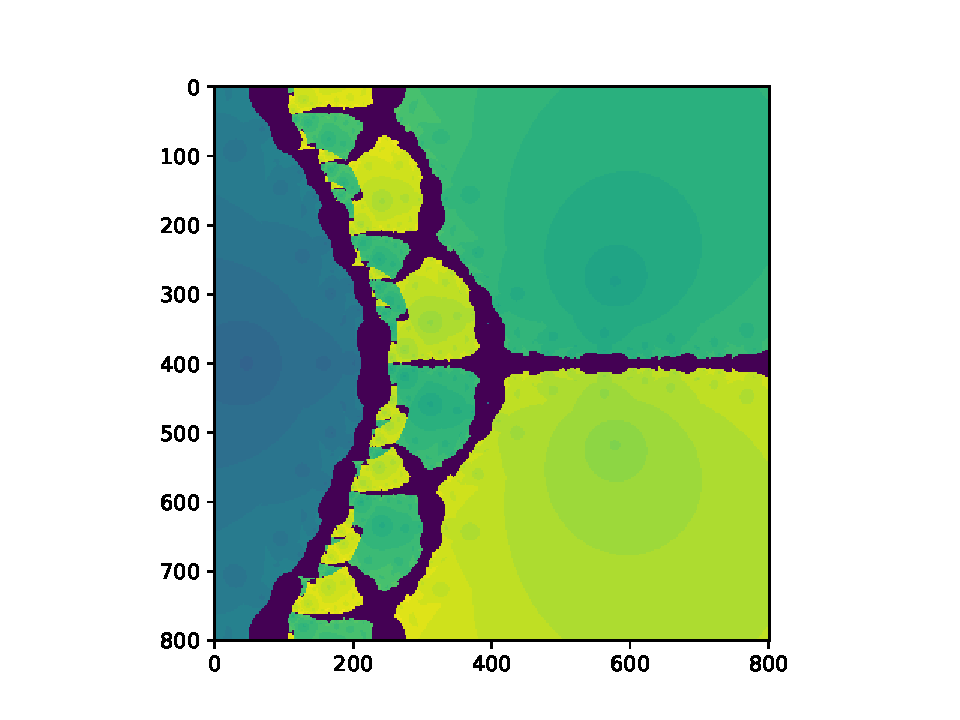
\includegraphics[scale=0.9]{out.pdf}
    \caption{Ausgabe für $x^3-2x+2$ auf dem Gebiet $[-2,2]\times[-2i,2i]$.}
    \label{3zeros}
\end{figure}
\begin{figure}
    \centering
    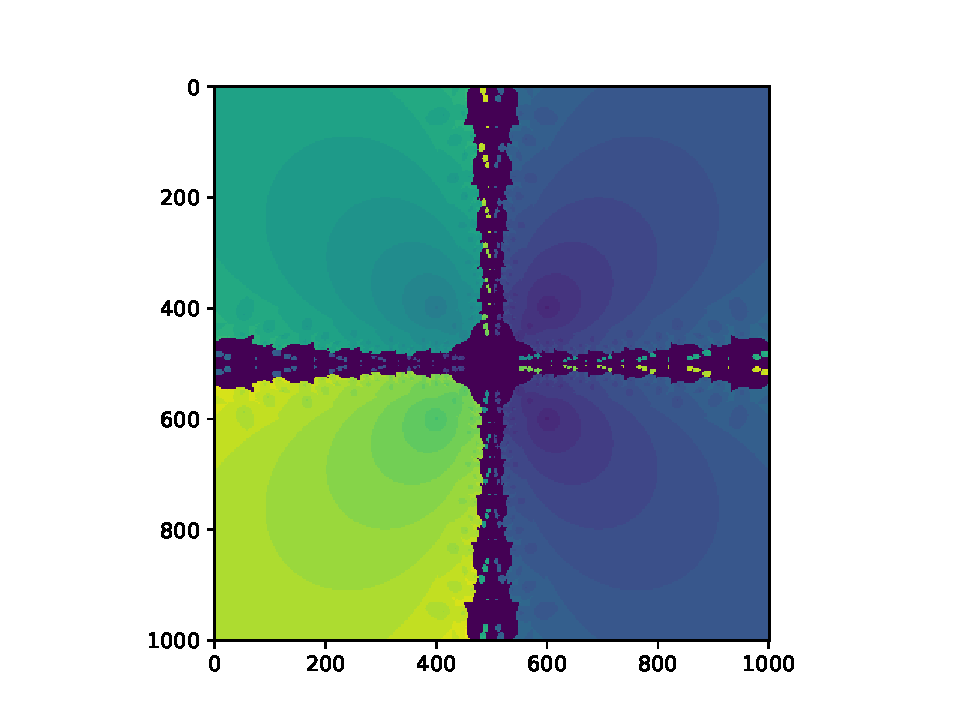
\includegraphics[scale=0.9]{out2.pdf}
    \caption{Ausgabe für $x^4+4$ auf dem Gebiet $[-5,5]\times[-5i,5i]$.}
    \label{4zeros}
\end{figure}
\end{document}